%!TEX root = notas_de_clase.tex

\section{Aprendizaje No Supervisado}

\subsection{Reducción de dimensionalidad}
\subsubsection{Principal Component Analysis (PCA)}
Formalmente, consideremos una matriz de datos $\hat{X}$:

$$
\hat{X}=\begin{bmatrix}
        \hat{x}_{11}    & \dots & \hat{x}_{1m}  \\
        \vdots          & \ddots& \vdots        \\
        \hat{x}_{n1}    & \dots & \hat{x}_{nm}
        \end{bmatrix},
$$

\noindent donde cada columna representa una variable de proceso distinta (característica) y cada fila un instante de tiempo, observación o ejemplo. De este modo se tienen $m$ características, y $n$ ejemplos. Es altamente recomendable que los datos de PCA estén normalizados, de modo que la normalización estará dada por:

\begin{equation*}
\hat{x}_{ij} = \frac{x_{ij}-\mu_j}{\sigma_{j}}
\end{equation*}

La dirección de mayor variabilidad está dada por los vectores propios de la \emph{matriz de covarianza empírica}:

\begin{align}
\Sigma & = \frac{1}{n-1}\hat{X}^T\hat{X}= V\Lambda V^T
\end{align}

donde $V$ es la matriz donde cada columna es un vector propio y $\Lambda$ es la matriz de valores propios. Un mayor valor para un valor propio indica mayor variabilidad para el vector propio asociado. Finalmente, los datos proyectados se pueden escribir como:

\begin{equation}
    X_{\text{proy}} = \hat{X}V
\end{equation}
Notemos que la transformación PCA es una rotación lineal de los datos.

Como observación, PCA encuentra una nueva base ortogonal tal que las componentes maximicen la variabilidad, esto implica que se pierde la intepretabilidad de las nuevas características generadas. A pesar de esto, utilizando las primeras 2 o 3 componentes PCA se pueden visualizar datos de alta dimensionabilidad.

Como se dijo anteriormente, es recomendable que las variables estén normalizadas, esto tiene justificación principalmente en evitar que las variables se vean afectadas por efectos de la escala. Por ejemplo, si tenemos dos variables temperatura en un rango de $0^\circ$C a $100^\circ$C, mientras que otra variable es la altura que va de $0$m a $10$m, notamos que claramente la variable temperatura aportará mayor variabilidad al sistema.
\subsubsection{Kernel PCA}
El método Kernel PCA es similar a PCA, pero esta vez se utiliza el truco del kernel para proyectar los datos. En ese sentido, en vez de calcular la matriz de covarianza empírica, se utiliza la matriz de Gram.

$$
K_{ij} = K(x_i,x_j) = \phi(x_i)\phi(x_j)^T
$$

Luego, se prosigue de la misma forma que PCA linear.

En la figura \ref{fig:kpca} se puede observar un ejemplo en que el resultado de PCA linear no es suficiente, puesto que el problema es simétrico, mientras que KPCA realiza una correcta separación de ambos clusters.

\begin{figure}[ht]
    \centering
    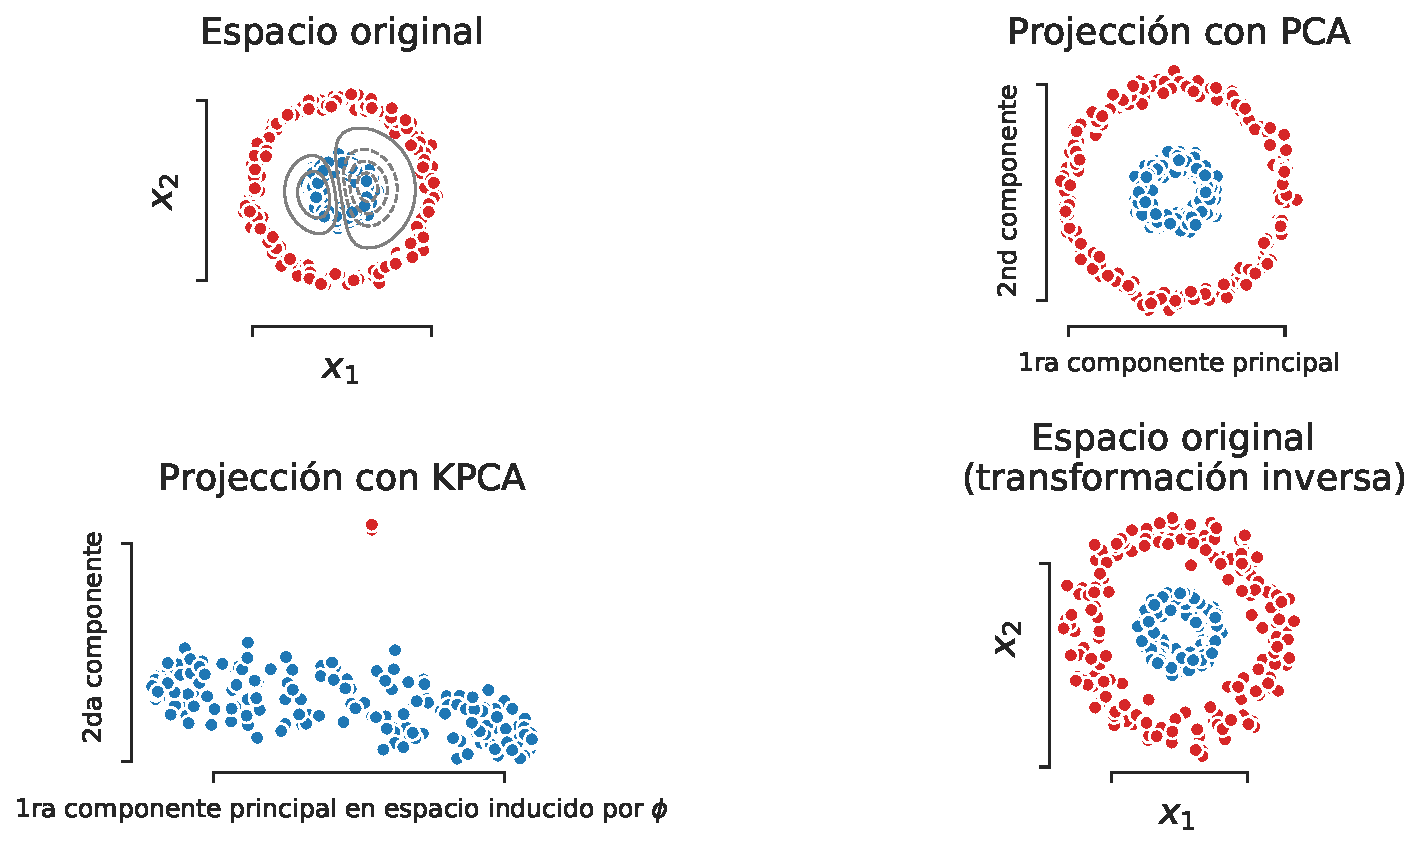
\includegraphics[width=0.7\linewidth]{img/cap7_kpca.pdf}
    \caption{Ejemplo en que kernel PCA sobre un conjunto de datos que no es linealmente separable.}
    \label{fig:kpca}
\end{figure}

\subsubsection{Probabilistic PCA}
PCA probabilístico (PPCA, por su sigla en inglés) tiene su inspiración en que PCA se puede expresar como la solución via máxima verosimilitud de un modelo probabilístico de variable latente. De este modo, PPCA propone un método iterativo para obtener la solución evaluando solo cierto número de componentes, sin necesidad de calcular la matriz de covarianza empírica.

El modelo probabilístico para PCA en que se inspira PPCA es el siguiente:

Sea $x_i\in \mathbb{R}^m$ los elementos observados, inputs o variables y $z\in \mathbb{R}^l$ una variable latente explícita correspondiente al espacio de las componentes principales. Se define un prior para $z$:

\begin{equation}
p(z) = N(0,I)
\end{equation}

De este modo, la distribución condicional de x dado z también es Gaussiana:

\begin{equation}
p(x|z) = N(Wz+\mu,\sigma^2I)
\end{equation}
Donde $W\in \mathbb{R}^{M\times l}$ y $\mu \in \mathbb{R}^m$ son parámetros a determinar. Notemos que no se pierde generalidad tomar el prior para $z$ con media cero y varianza unitaria, puesto que si se toma otro prior más general, se produce el mismo modelo.

Dado que tenemos modelo paramétrico probabilístico, podemos estimar los parámetros con máxima verosimilitud. Dado los datos $X = \{x_i\}_{i=1}^n$. La log-verosimilitud está dada por:

\begin{align}
\log p(X|W,\mu, \sigma^2) & = \sum_{i=1}^n \log p(x_i|W,\mu, \sigma^2)\\
& = \frac{n l}{2}\log (2\pi) - \frac{n}{2}log|C| - \frac{1}{2}\sum_{i=1}^n (x_i-\mu)^T C^{-1} (x_i-\mu),
\end{align}

con $C = WW^T + \sigma^2 I$.

Usando la condición de primer orden obtenemos

\begin{align}
\mu = \bar{x} = \frac{1}{n}\sum_{i=1}^n x_i.
\end{align}
De esta manera tenemos la función de log-verosimilitud completa:

\begin{align}
    \log p(X, Z|W, \mu, \sigma^2) = \sum_{i=1}^n \{\log p(x_i|z_i) + \log p(z_i)\}
\end{align}

y evaluando en $\mu = \bar{x}$

\begin{align}
\notag \mathbb{E}[ p(X,Z |W, \mu, \sigma^2) ] =  -\sum_{i=1}^n \Bigg\{ &\frac{l}{2} \log (2\pi \sigma^2)\\
\notag & + \frac{1}{2}\text{Tr}(\mathbb{E}[z_iz_i^T])\\
\notag & \frac{1}{2\sigma^2}||x_i - \mu||^2 - \frac{1}{\sigma^2}\mathbb{E}[z_i]^T W^T (x_i - \mu)\\
& \frac{1}{2\sigma^2} \text{Tr}(\mathbb{E}[z_iz_i^T]W^T W) \Bigg\}
\end{align}

\section{Clustering}

\subsection{k-means}
Dado un entero $k \in \mathbb{N}$ y uin conjunto de observaciones $X = \{x_i\}_{i=1}$ con $x_i\in \mathbb{R}^D$ queremos separar los datos en k graupos, donde cada grupo se le asigna un centroide $\mu_k$ y cada elemento $x_i$ se le asigna el grupo que tenga el centroide más cercano.

Sea $r_{ik}$ la asignación, esta estará definida por:

\begin{align*}
r_{ik} = \begin{cases}
1 & \text{si } k = \text{argmin}||x_i-x_k||\\
0 & \text{si no.}
\end{cases}
\end{align*}
Es decir, para encontrar los centroides se debe minimizar la función:

\begin{align}
J = \sum_{i=1}^N \sum_{k=1}^K r_{ik} ||x_i-x_j||^2
\end{align}

Para minimizar esta función utilizaremos un enfoque llamado \emph{Expectation-Maximization}. Este es un método iterativo y como tal, tiene problemas con mínimo locales, pero para solucionar esto, basta inicializar el algoritmo muchas veces.

El algoritmo está dado por:

\begin{itemize}
    \item \textbf{E-step:} En este paso, se calculan (actualizan) las asignaciones $r_{ik}$, dejando fijos $\mu_k$. Lo que corresponde a asignar el dato $x_i$ al centroide más cercano.
    \item \textbf{M-step:} El siguiente paso corresponde a actualizar los centroides $\mu_k$ dejando fijo las asignaciones $r_{ik}$.
    
    Como J es cuadrática en $\mu_k$, entonces podemos utilizar la condición de primer orden:
    \begin{align}
        \mu_k = \frac{\sum_{i=1}^N r_{ik}x_i}{\sum_{i=1}^N r_{ik}}
    \end{align}
    
    Lo que corresponde a asignar el centro del cluster al promedio de todas las muestras asignadas al antiguo cluster.
\end{itemize}

\underline{\textbf{Ejemplo:}} En la figura \ref{fig:kmeans} se observa un ejemplo de clustering utilizando kmeans. Como se puede notar, los clusters creados por kmeans son circulares, puesto que se utiliza distancia euclediana hace el centro del cluster.

\begin{figure}[ht]
  \centering
  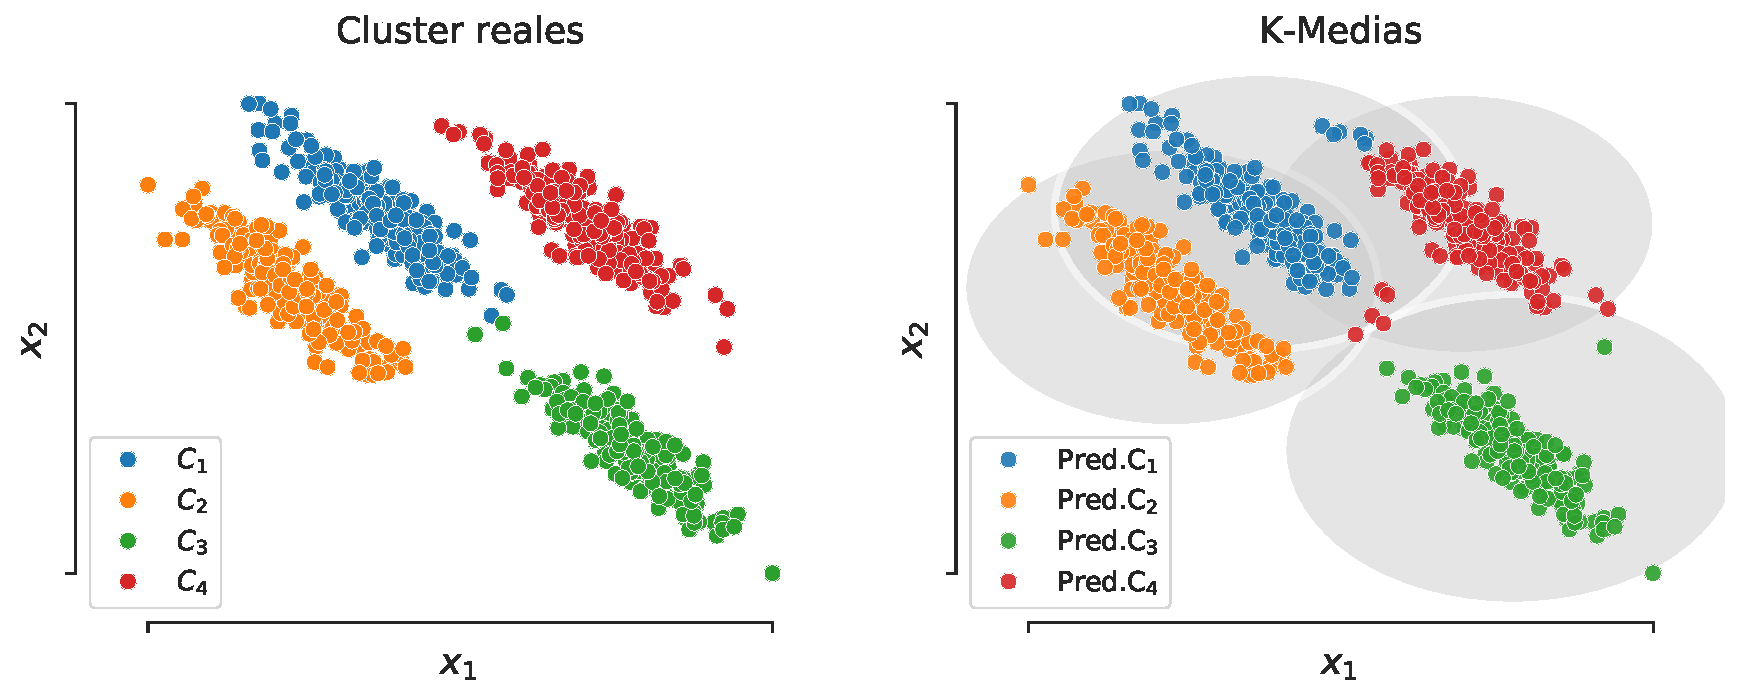
\includegraphics[width=0.8\textwidth]{img/cap7_k_medias}
  \caption{(Izquierda) Datos reales con sus etiquetas correctas. (Derecha) Clusters encontrados por k-means.}
  \label{fig:kmeans}
\end{figure}

\subsection{Gaussian Mixture Model}

La mezcla de gaussianas (GMM por su sigla en inglés) es un caso general de k-means, en donde no solo ajustamos los centros (vector de medias $\mu_k$) si no también el modelo considera matrices de covarianza $\Sigma_k$. En ese sentido, se puede interpretar k-means como el caso particular en que $\Sigma_k = I$ y asignación directa (\emph{hard labeling)}.

En el modelo de GMM se tiene que la probabilidad de una muestra, dado nuestro modelo de mezcla de gaussianas es:

\begin{align}
p(x_i|\theta) = \sum_{k=1} \pi_k \mathcal{N}(x_i| \mu_k,\Sigma_k)
\end{align}
donde:

\begin{align}
\mathcal{N}(x_i| \mu_k,\Sigma_k) = \frac{1}{(2\pi)^{D/2}|\Sigma|^{1/2}}\exp \left[ -\frac{1}{2}(x_i-\mu_k)^T \Sigma_k^{-1}(x_i-\mu_k) \right]
\end{align}
y $\pi_k$ son los pesos de las mezclas. La forma de encontrar los parámetros es la misma que en k-means, solo que esta vez en el paso de maximización, se debe estimar $\mu_k$, $\Sigma_k$ y $\pi_k$.

Esto se resume como:

\begin{itemize}
    \item \textbf{E-step:} Evaluamos las probabilidades posteriores:
    
    \begin{align}
    r_{ik} = \frac{\pi_k \mathcal{N}(x_i| \mu_k,\Sigma_k)}{\sum_{k'=1}^K \pi_{k'}\mathcal{N}(x_i| \mu_{k'},\Sigma_{k'})}
    \end{align}
    \item \textbf{M-step:} Se re-estiman los parámetros, usando:
    \begin{align}
    \mu_k^{new} & = \frac{1}{R_k}\sum_{i=1}^N r_{ik}x_i\\
    \Sigma_k^{new} & = \frac{1}{R_k} \sum_{i=1}^N r_{ik}(x_i - \mu_k^{new})(x_i - \mu_k^{new})^T\\
    \pi_k^{new} & = \frac{R_k}{R}
    \end{align}
    Donde
    \begin{align*}
    R_k = \sum_{i=1}^N r_{ik} \qquad \text{y} \qquad R = \sum_{k=1}^K R_k.
    \end{align*}
    El criterio de detención es evaluar la función de verosimilitud hasta que converja.
\end{itemize}

\underline{\textbf{Ejemplo:}} La figura \ref{fig:gmm} muestra un ejemplo de clustering utilizando GMM. En este caso, se puede observar directamente como GMM es una generalización de kmeans, en donde ahora los clusters tienen forma de gaussiana anisotrópica.

\begin{figure}[ht]
  \centering
  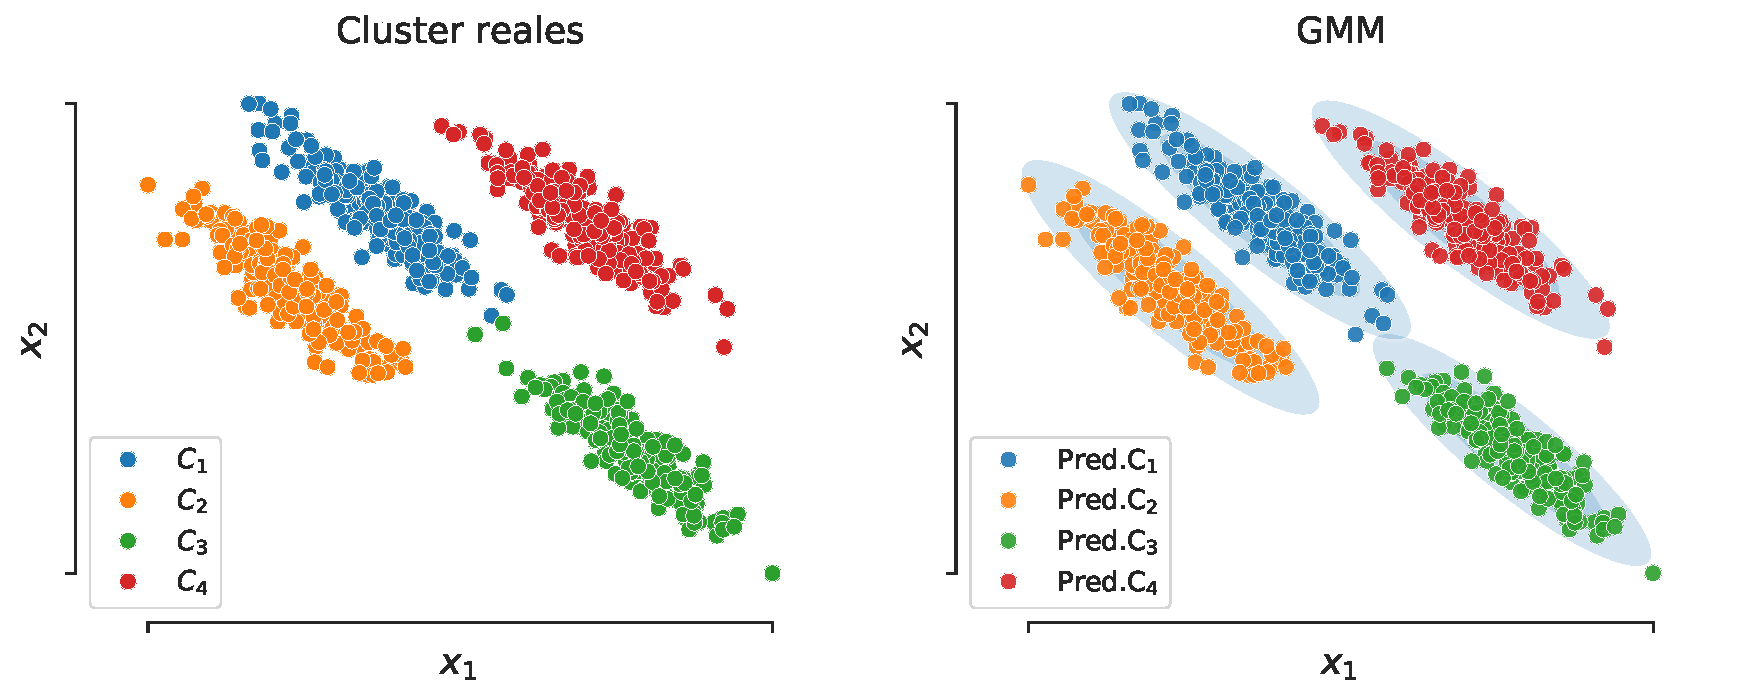
\includegraphics[width=0.8\textwidth]{img/cap7_gmm}
  \caption{(Izquierda) Datos reales con sus etiquetas correctas. (Derecha) Clusters encontrados por GMM.}
  \label{fig:gmm}
\end{figure}


\subsection{Density-based spatial clustering of applications with noise (DBSCAN)}

Es un algoritmo de clustering propuesto por Martin Ester et al. el cual ha tenido mucha popularidad puesto que no requiere definir una cantidad inicial de número de clusters. Los hiper-parámetros de entrada del modelo son 2:

\begin{itemize}
    \item Mínimo número de punto $minPts$.
    \item Radio o vecindad $\epsilon$.
\end{itemize}

El algoritmo se basa en la idea de que dado 2 púntos $x_i$, $x_j$ dentro de un mismo cluster, se dice que \emph{$x_i$ es alcanzable por $x_j$}, si siempre se puede llegar de $x_i$ a $x_j$ avanzando de punto en punto, donde la distancia entre cada uno es al menos menor que $\epsilon$ y además un punto intermedio es un punto núcleo. Con estos el algoritmo define tres tipos de puntos:

\begin{itemize}
    \item \textbf{Puntos núcleo:} Son puntos $x_i$ tales que en una vecindad $\epsilon$ tienen almenos $minPts$ vecinos.
    \item \textbf{Puntos borde:} Constituyen el \textit{borde externo} de los cluster.
    \item \textbf{Outliers:} Puntos que no son alcanzables por ningún punto.
\end{itemize}

Notemos que con lo anterior, se desprende que todo cluster debe tener al menos un punto núcleo.
El algoritmo para encontrar los clusters es el siguiente:


\begin{algorithm}[H]
  \caption{Pseudo código de DBSCAN
    \label{DBSCAN}}
  \begin{algorithmic}[1]
    \Function{DBSCAN}{$D, eps, MinPts$}
      \State $C \gets 0$\;
      \For{{cada punto $P$ no visitado en $D$}}
      \State marcar $P$ como visitado
        \If{sizeOf(PuntosVecinos) $\le$ MinPts}
        \State marcar $P$ como RUIDO
        \Else
        \State C $\gets$ C+1
        \State expandirCluster(P,vecinos, C, eps, MinPts)
        \EndIf
      \EndFor
    \EndFunction
  \end{algorithmic}
\end{algorithm}


\begin{algorithm}[H]
  \caption{Función para expandir cluster.
    \label{alg:expandirCluster}}
  \begin{algorithmic}[1]
  \Function{expandirCluster}{P, vecinosPts, C, eps, MinPts}
  \State agregar P al cluster C
  \For{cada punto P' en vecinosPts}
  \If{P' no fue visitado}
         \State marcar P' como visitado\;
         \State vecinosPts' $\gets$ regionDeConsulta(P', eps)\;
         \If{sizeof(vecinosPts') $\geq$ MinPts}
            \State vecinosPts $\gets$ vecinosPts $\cup$ vecinosPts'
        \EndIf
    \EndIf
    \If{P' no tiene cluster asignado}
         \State P' se le asigna el cluster C
    \EndIf
    \EndFor
    \EndFunction
  \end{algorithmic}
\end{algorithm}


\begin{algorithm}[H]
  \caption{Retorna los puntos de la vecindad de búsqueda para un punto.
    \label{alg:regionDeConsulta}}
  \begin{algorithmic}[1]
    \Function{regionDeConsulta}{$P, eps$}
    
    \Return Todos los puntos junto a P' que están a eps de distancia (incluyendo P)
    \EndFunction
  \end{algorithmic}
\end{algorithm}


\underline{\textbf{Ejemplo:}} La figura \ref{fig:dbscan} muestra un ejemplo de clustering utilizando DBSCAN. La figura \ref{fig:dbscan}(derecha) muestra en negro los puntos que son clasificados como ruido o \emph{outliers} por el algoritmo. Por otro lado, los puntos núcleos son graficados como un punto grande, mientras que los puntos borde se grafican con un marcador pequeño.

\begin{figure}[H]
  \centering
  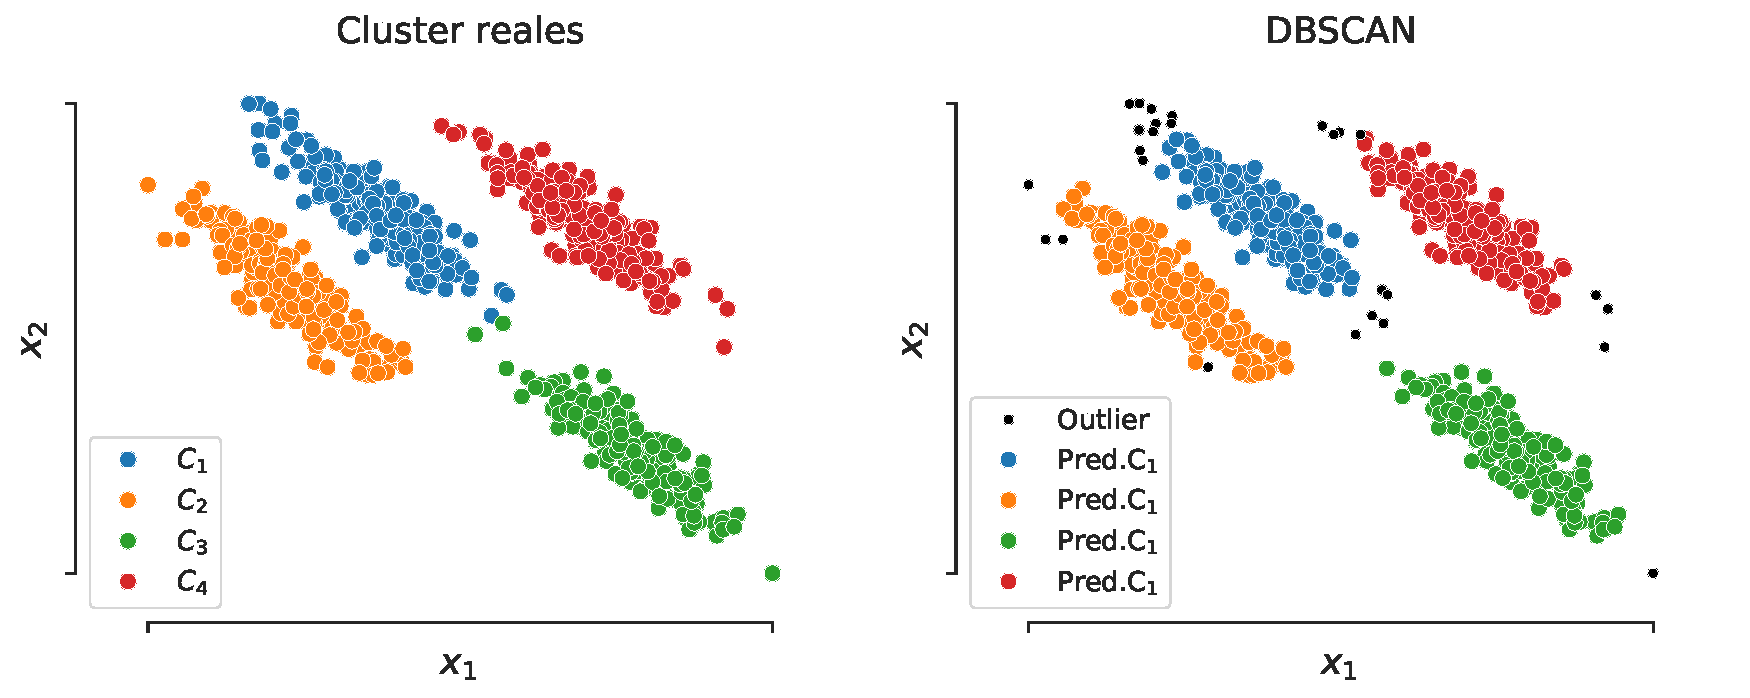
\includegraphics[width=0.8\textwidth]{img/cap7_dbscan}
  \caption{(Izquierda) Datos reales con sus etiquetas correctas. (Derecha) Clusters encontrados por DBSCAN.}
  \label{fig:dbscan}
\end{figure}